\documentclass{article}

\usepackage{color}
\definecolor{dkgreen}{rgb}{0,0.6,0}
\definecolor{gray}{rgb}{0.5,0.5,0.5}
\definecolor{mauve}{rgb}{0.58,0,0.82}
\usepackage[margin=1in]{geometry}
\usepackage{fancyhdr}
\pagestyle{fancy}
\lhead{\today}
\chead{Ying Qiao SID:21412301}
\rhead{Stat215B Sp13: Assignment 6}
\lfoot{}
\cfoot{\thepage}
\rfoot{}
\usepackage{graphicx}
\usepackage{textcomp}
\usepackage{lmodern}
\usepackage[T1]{fontenc}
\usepackage{listings}
\usepackage{amssymb,amsmath}
\usepackage{bm}
\usepackage{hhline}

%% for inline R code: if the inline code is not correctly parsed, you will see a message
\newcommand{\rinline}[1]{SOMETHING WORNG WITH knitr}
%% begin.rcode setup, include=FALSE
% opts_chunk$set(fig.path='figure/latex-', cache.path='cache/latex-')
%% end.rcode


\begin{document}
\section*{Math stats}
Efron (2010) exercises

\subsubsection*{2.5}
Within Lemma 2.1, we have two expectations of functions
\begin{displaymath}
\begin{split}
E\{\overline{Fdr}(\mathcal{Z}) | N_1(\mathcal{Z})\} 
& = E\{ \frac{e_0(\mathcal{Z})}{N_0(\mathcal{Z}) + N_1(\mathcal{Z})} |N_1(\mathcal{Z})\}
= E\{ \eta(N_0(\mathcal{Z})) | N_1(\mathcal{Z}) \} \\
E\{Fdp(\mathcal{Z}) | N_1(\mathcal{Z})\} 
& = E\{ \frac{N_0(\mathcal{Z})}{N_0(\mathcal{Z}) + N_1(\mathcal{Z})} |N_1(\mathcal{Z})\}
= E\{ \zeta(N_0(\mathcal{Z})) | N_1(\mathcal{Z}) \}
\end{split}
\end{displaymath}
where $\eta(N_0(\mathcal{Z}))$ is convex and $\zeta(N_0(\mathcal{Z}))$
is concave.
\subsubsection*{}
Meanwhile, we have one function of expectations
\begin{displaymath}
\phi_1(\mathcal{Z}) = \frac{e_0(\mathcal{Z})}{e_0(\mathcal{Z}) + N_1(\mathcal{Z})}
\end{displaymath}
here, with null case independence,
\begin{displaymath}
e_0(\mathcal{Z}) = E\{ N_0(\mathcal{Z}) \} = E\{ N_0(\mathcal{Z}) | N_1(\mathcal{Z})\}
\end{displaymath}
Then, we have
\begin{displaymath}
\begin{split}
\phi_1(\mathcal{Z}) &= \frac{e_0(\mathcal{Z})}{E\{N_0(\mathcal{Z})\} +  N_1(\mathcal{Z})} 
= \eta(E\{N_0(\mathcal{Z}) | N_1(\mathcal{Z})\}) \\
\phi_1(\mathcal{Z}) &= \frac{E\{N_0(\mathcal{Z})\}}{E\{N_0(\mathcal{Z})\} +  N_1(\mathcal{Z})} 
= \zeta(E\{N_0(\mathcal{Z}) | N_1(\mathcal{Z})\})
\end{split}
\end{displaymath}
Finally, with different function conditions for Jensen's inequality,
we have:\newline
for convex $\eta(\cdot)$,
\begin{displaymath}
\begin{split}
\eta(E\{N_0(\mathcal{Z}) | N_1(\mathcal{Z})\}) &\leq E\{\eta(N_0(\mathcal{Z})) | N_1(\mathcal{Z}) \} \\
\leftrightarrow
\phi_1(\mathcal{Z}) &\leq E\{\overline{Fdr}(\mathcal{Z}) | N_1(\mathcal{Z})\} 
\end{split}
\end{displaymath}
for concave $\zeta(\cdot)$,
\begin{displaymath}
\begin{split}
\zeta(E\{N_0(\mathcal{Z}) | N_1(\mathcal{Z})\}) &\geq E\{\zeta(N_0(\mathcal{Z})) | N_1(\mathcal{Z}) \} \\
\leftrightarrow
\phi_1(\mathcal{Z}) &\geq E\{Fdp(\mathcal{Z}) | N_1(\mathcal{Z})\} 
\end{split}
\end{displaymath}
That completes our proof for (2.30).


\subsubsection*{4.1}
In this frequentist multiple testing situation, we condition on fixed
$N_0$ null cases and $N_1$ non-null cases ($N_0,N_1 > 0$).
Here, we define test $i$ size $\alpha_i$ ($i \in I_0, |I_0|=N_0$) and
test $j$ power $\beta_j$ ($j \in I_1, |I_1| = N_1$), 
with $\{1,...,N\} = I = I_0 \bigcup I_1$, as,  
\begin{displaymath}
\begin{split}
\alpha_i &= Pr\{a_i = 1 | H_{0i} \hspace{4 pt} true\} = E\{a_i | i\in I_0\}\\
\beta_j &= Pr\{b_j = 1 | H_{1j} \hspace{4 pt} true\} = E\{b_j | j\in I_1\}
\end{split}
\end{displaymath}
where
\begin{displaymath}
a = \sum_{i\in I_0} a_i, \hspace{4 pt} b = \sum_{j \in I_1} b_j
\end{displaymath}
So, now we have
\begin{displaymath}
\begin{split}
E\{\frac{a}{N_0}\} & = \frac{1}{N_0} \sum_{i\in I_0} E\{a_i | i\in I_0\} 
= \frac{1}{N_0} \sum_{i\in I_0} \alpha_i = \bar{\alpha} \\
E\{\frac{b}{N_1}\} & = \frac{1}{N_1} \sum_{j\in I_1} E\{b_j | j\in I_1\} 
= \frac{1}{N_1} \sum_{j\in I_1} \beta_i = \bar{\beta} 
\end{split}
\end{displaymath}


\subsubsection*{4.2}
Conditioned on $R$, $R>0$, we get
\begin{displaymath}
a = \sum_{i\in I_R} a_i
\end{displaymath}
where 
\begin{displaymath}
I_R \subset I = \{1,...,N\}, |I_R| = R
\end{displaymath}
Also, from the setting, we have the two-groups model, $i.i.d.$ $z_i, i=1,...,N$
\begin{displaymath}
\begin{split}
Pr\{H_{0i}\}=\pi_0; \hspace{6 pt} z_i | H_{0i} &\sim f_0, F_0 \\
Pr\{H_{1i}\}=\pi_1; \hspace{6 pt} z_i | H_{1i} &\sim f_1, F_1 \\
\rightarrow z_i &\sim f,F \\
&f=\pi_0f_0+\pi_1f_1; F=\pi_0F_0 + \pi_1F_1
\end{split}
\end{displaymath}
Meanwhile, the decision rule rejects $H_{0i}$ for $z_i \in \mathcal{Z}$, i.e.,
\begin{displaymath}
\{i \in I_R\} \leftrightarrow \{z_i \in \mathcal{Z} \}
\end{displaymath}
So, for each $a_i$, it is a Bernulli variable with the same probability $p$,
\begin{displaymath}
\begin{split}
p &= Pr\{ a_i=1 | i\in I_R \} \\
&= Pr\{ H_{0i} | z_i\in \mathcal{Z} \} \\
&= \frac{Pr\{ H_{0i} \} \cdot Pr\{ z_i\in \mathcal{Z} | H_{0i}\}}{Pr\{ z_i\in \mathcal{Z} \}} \\
&= \frac{\pi_0 F_0(\mathcal{Z})}{F(\mathcal{Z})} \\
&= Fdr(\mathcal{Z}) = \phi(\mathcal{Z})
\end{split}
\end{displaymath}
Naturally, we get
\begin{displaymath}
\begin{split}
a_i \sim^{i.i.d.} Bern(\phi(\mathcal{Z})) \\
\rightarrow a =\sum_{i\in I_R} a_i \sim Bi(R, \phi(\mathcal{Z})) 
\end{split}
\end{displaymath}
Finally, we have the scaled version
\begin{displaymath}
a/R \sim Bi(R, \phi(\mathcal{Z}))/R
\end{displaymath}
 

\subsubsection*{4.4}
Theorem 4.1: \newline
For independent $p$-value $p_i$ of each testing case $i$, rule BH($q$) rejects
\begin{displaymath}
H_{0(1)}, ... , H_{0(i_{max})}
\end{displaymath}
and accept others, where $(i)$ are the ordered indices
\begin{displaymath}
p_{(1)} \leq p_{(2)} \leq ... \leq p_{(i)} \leq ... \leq p_{(N)}
\end{displaymath}
and for a fixed value of $q$,
\begin{displaymath}
i_{max} \equiv max\{i | p_{(i)} \leq \frac{i}{N}q  \}
\end{displaymath}
This leads to that, $\pi_0 = N_0 / N$,
\begin{displaymath}
E\{ Fdp_{BH(q)} \} = \pi_0q
\end{displaymath}
Corollary 4.2:\newline
For independent real-valued test statistics $z_i$, without of loss of
generality, corresponding to left-tailed $p$-value $p_i$, ($i=1,...,N$)
\begin{displaymath}
p_i = F_0(z_i) \hspace{8 pt} \leftrightarrow \hspace{8 pt} z_i = F_0^{-1}(p_i)
\end{displaymath}
where, for all $i$, $z_i | H_{(0i)} \sim f_0, F_0$ and $z_i \sim f, F$, 
empirical CDF $\bar{F}(z) = \# \{z_i\leq z \}/N$.\newline
Rule EB($q$) rejects
\begin{displaymath}
H_{0(1)}, ... , H_{0(i_{max})}
\end{displaymath}
and accpet others, where $(i)$ are the ordered indices equivalent to those $p_{(i)}$ indices
\begin{displaymath}
z_{(1)} \leq z_{(2)} \leq ... \leq z_{(i)} \leq ... \leq z_{(N)}
\end{displaymath}
and for a fixed $q$,
\begin{displaymath}
i_{max} \equiv max\{ i | \overline{Fdr}(z_{(i)}) \leq q \}
\end{displaymath}
The condition here is equivalent to BH($q$) in that
\begin{displaymath}
\begin{split}
\overline{Fdr}(z_{(i)}) &\leq q \\
\frac{\pi_0F_0(z_{(i)})}{\bar{F}(z_{(i)})} &\leq q \\
\frac{\pi_0p_{(i)}}{i/N} &\leq q \\
p_{(i)} &\leq \frac{i}{N} \frac{q}{\pi_0}
\end{split}
\end{displaymath}
So, even $\pi_0$ is unknown, with the equivalency to Theorem
4.1, we can see that
\begin{displaymath}
E\{ Fdp_{EB(q)} \} = \pi_0 \frac{q}{\pi_0} = q
\end{displaymath}


\subsubsection*{4.5}
In Figure 4.3, we are plotting $\overline{Fdr}(z)$, $\overline{Fdr}^{(c)}(z)$ vs. $z$-values,
\begin{displaymath}
\begin{split}
\overline{Fdr}(z) &= \pi_0F_0(z) / \bar{F}(z) \\
\overline{Fdr}^{(c)}(z) &= \pi_0F_0^{(c)}(z) / \bar{F}^{(c)}(z)
\end{split}
\end{displaymath}
where $z_i | H_{0i} \sim F_0$, $z_i \sim F$ and the complementary CDF
$F^{(c)}(z)= 1 - F(z)$. \newline
Here, for left-sided tests, when $z$ is positively large ($z>3$),
\begin{displaymath}
\bar{F}(z) \rightarrow F_0(z);
\overline{Fdr}(z) \rightarrow \pi_0
\end{displaymath}
Similarly, for right-sided tests, when $z$ is negatively large ($z<-3$),
\begin{displaymath}
\bar{F}^{(c)}(z) \rightarrow F_0^{(c)}(z);
\overline{Fdr}^{(c)}(z) \rightarrow \pi_0
\end{displaymath}
When setting $\pi_0 = 1$, we should see that
\begin{displaymath}
\begin{split}
\overline{Fdr}(z) \simeq 1, &\hspace{4 pt} z>3 \\
\overline{Fdc}^{(c)}(z) \simeq 1, &\hspace{4 pt} z<-3 
\end{split}
\end{displaymath}
as shown up in Figure 4.3.


\subsubsection*{4.6}
From the $z$-value histogram of Efron Figure 2.1 and Figure 3.1, we
can see that the prostate data is more \textit{symmetrical} than the
DTI data, with respect to null standard normal distribution. The DTI
data actually has two half-brain data, which is more heavily tailed to
the right than to the left, making the two-sided testing results
rejecting fewer cases.
\begin{figure}
\begin{center}
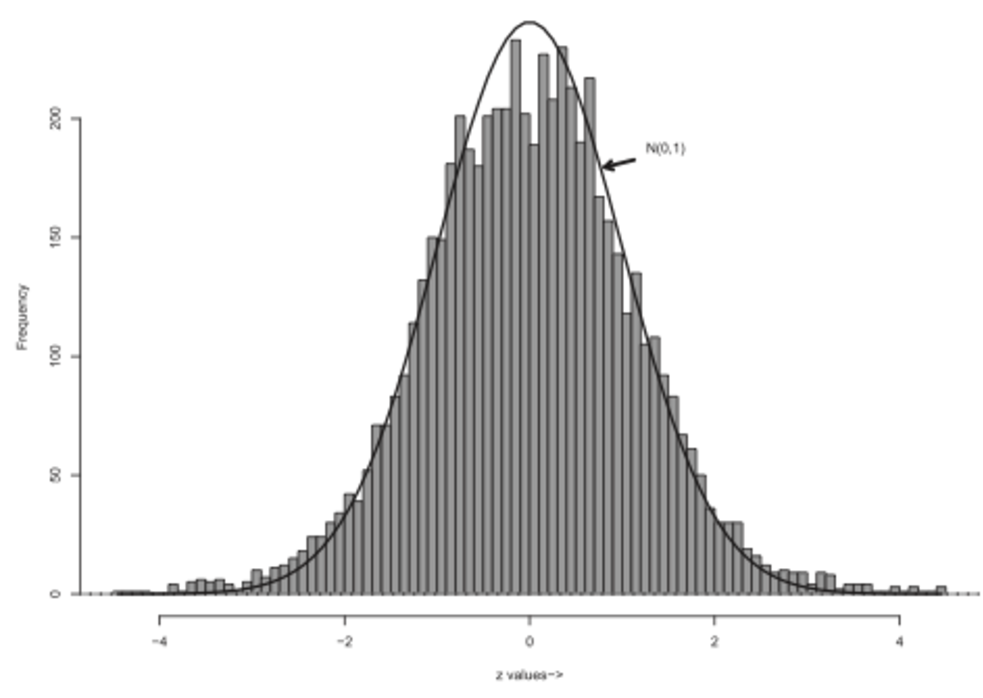
\includegraphics[height=2in,width=4in]{Fig21}
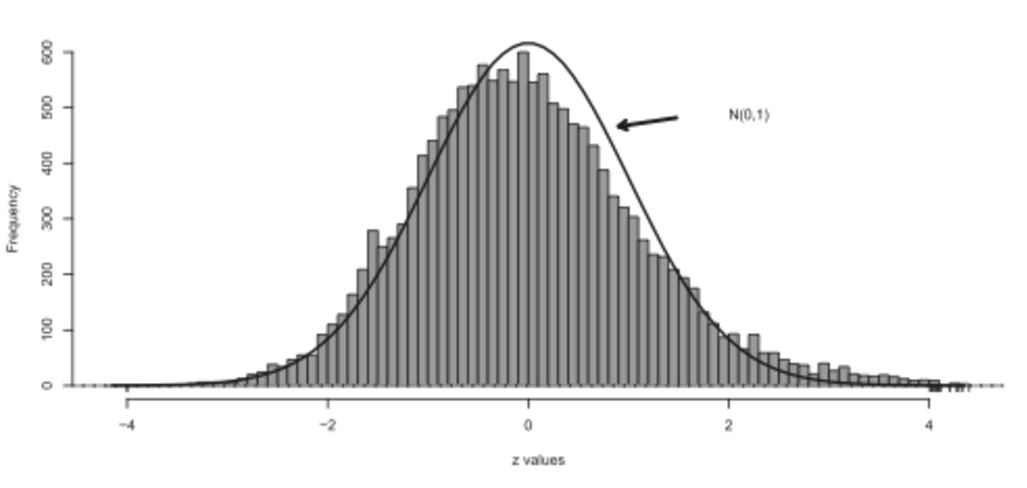
\includegraphics[height=2in,width=4in]{Fig31}
\caption{Efon Figure2.1 (top) and Figure3.1 (bottom)}
\end{center}
\end{figure}
So, the results summerized in the table show that the two-sided testing of the
prostate data are less wasteful. 
\begin{center}
\begin{tabular}{l|lll} \hline
$R_{BH(0.1)}(Z)$ & left-tailed & right-tailed & two-tailed  \\ \hline
prostate & 32($z_i\leq -3.26$) & 28($z_i\geq 3.36$) & 60($|z_i|\geq 3.29$) \\
DTI        & 0                              & 192($z_i\geq 3.02$) & 110
\end{tabular}
\end{center}





\newpage
\section*{Prostate microarray data}
\hspace{12 pt} We have the prostate microarray data from the Efron
book, a $6033 \times 102$ matrix $X=\{x_{ij}\}$.
\begin{center}
$x_{ij}$ = expression of gene $i$ on patient $j$, 
\end{center}
where $i=1,..,N$, $N=6033$; normal patients $j=1,...,50$ vs. cancer
patients $j=51,...,102$.
%%  begin.rcode ass6-00,cache=TRUE,results="markup",message=FALSE,echo=FALSE
%%rm(list=ls())
%%load("prostatedata.Rda")
%%N <- dim(prostatedata)[1]
%%  end.rcode


\subsubsection*{Efron Figure 2.1}
\hspace{12 pt} The large-scale hypothesis testing that we perform on
this dataset use the two-sample $t$-statistic. \newline
For testing gene $i$,
\begin{displaymath}
t_i = \frac{\bar{x}_i(2) - \bar{x}_i(1)}{s_i}
\end{displaymath}
\begin{displaymath}
\bar{x}_i(1) = \frac{1}{50} \sum_{j=1}^{50} x_{ij} ; \hspace{8 pt}
\bar{x}_i(2) = \frac{1}{52} \sum_{j=51}^{102} x_{ij}
\end{displaymath}
\begin{displaymath}
s_i^2 = \frac{\sum_{j=1}^{50} (x_{ij} - \bar{x}_i(1))^2 +
  \sum_{j=51}^{102} (x_{ij} - \bar{x}_i(2))^2 }{100} \cdot (\frac{1}{50} + \frac{1}{52}) 
\end{displaymath}
Then, we transform to the $z$-values, 
where $\Phi$ is the standard normal CDF and $F_{100}$ is the Student-$t$ CDF
with 100 degrees of freedom,
\begin{displaymath}
z_i = \Phi^{-1}(F_{100}(t_i))
\end{displaymath}
Finally, we reproduce Efron
Figure 2.1, histogram of $z$-values testing $N=6033$ genes
for possible involvement with prostate cancer.

%%  begin.rcode ass6-21,cache=TRUE,echo=FALSE,results="markup",dev='pdf',fig.height=6,fig.width=7,fig.align="center",fig.cap="Reproduced Efron Figure 2.1"
%%x1 <- rowMeans(prostatedata[ ,1:50])
%%x2 <- rowMeans(prostatedata[ ,51:102])
%%s2 <- (1/50 + 1/52)/100 * (rowSums((prostatedata[ ,1:50] - x1)^2) + rowSums((prostatedata[ ,51:102] - x2)^2))
%%t <- (x2 - x1) / sqrt(s2)
%%z <- qnorm(pt(t, 100)) #greater
%%hist(z, breaks=100, xlim=c(-5,5), xlab="z values->", ylab="Frequency", main="", col="grey")
%%  end.rcode


\subsubsection*{Efron Figure 4.2}
\hspace{12 pt} We implement Benjamini and Hochberg's FDR control
algorithm here. Our right-sided testing for the prostate data
produces $p$-value $p_i$ for each case, 
\begin{displaymath}
p_i = F_{100}(-t_i)
\end{displaymath}
After ordering and choosing $q=0.1$, we reproduce Efron Figure 4.2. 

%%  begin.rcode ass6-42,cache=TRUE,echo=FALSE,results="markup",dev='pdf',fig.height=6,fig.width=7,fig.align="center",fig.cap="Reproduced Efron Figure 4.2"
%%q <- 0.1
%%p <- pt(-t, 100)
%%p.sort <- sort(p)
%%R <- length(p.sort[p.sort <= q/N*(1:N)])
%%plot(1:50, p.sort[1:50], typ="p", pch="*", col="black", xlab="index i", ylab="ordered p-values")
%%lines(x=1:50, y=q/N*(1:50), lwd=2)
%%  end.rcode

Here, stars indicate $p$-values for the 50 largest $z_i$, and the
solid line (slope=$q/N$) intersection gives us the \rinline{R}
rejections of the null cases under BH($q$) control. So among the
\rinline{R} non-null genes, the expected number of 
false discoveries should be \rinline{q*R}, which is quite good.

\end{document}
